\section{Discussion}
We claim that our implementation is correct-by-construction because the code \textit{is} the model specification - we have closed the gap between the specification and its implementation. Also we can guarantee that no non-deterministic influences can happening, neither in our nor Yampas library code due to the strong static type system of Haskell. This guarantees that repeated runs of the simulation will always result in the exact same dynamics given the same initial parameters, something of fundamental importance in System Dynamics. See Figure \ref{fig:sir_sd_visualisation} for a real-time visualisation of the SIR simulation of our Haskell implementation.

\begin{figure}
	\centering
	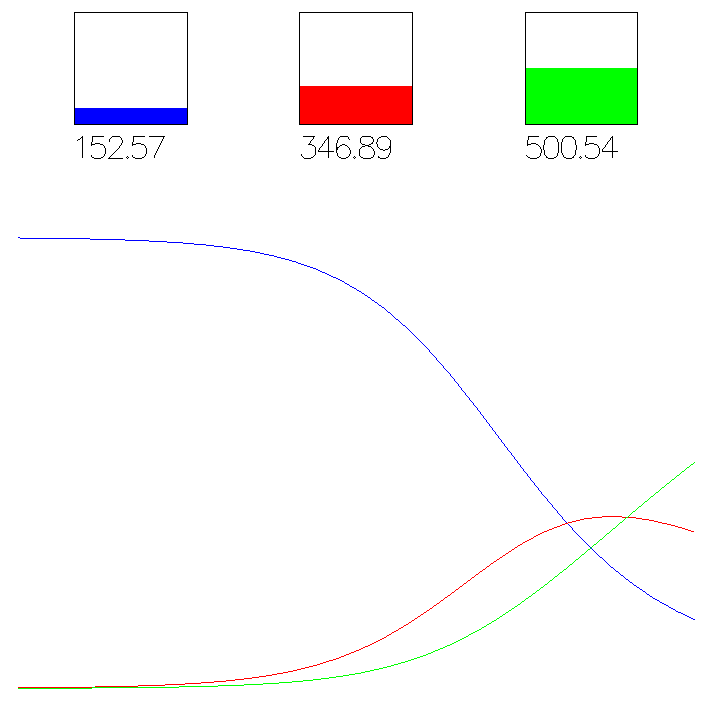
\includegraphics[width=.4\textwidth, angle=0]{./fig/visualisation_t50.png}
	\caption{Snapshot of a real-time visualisation of a SIR compartment model simulating using Haskell at $t = 50$. Population Size $N$ = 1,000, contact rate $\beta = \frac{1}{5}$, infection probability $\gamma = 0.05$, illness duration $\delta = 15$ with initially 1 infected agent. TODO: explain stocks and add axes}
	\label{fig:sir_sd_visualisation}
\end{figure}

\subsection{Results}
Although we have translated our model specifications directly into code we still we need to validate the dynamics and test the system for its numerical behaviour under varying $\Delta t$. This is necessary because numerical integration, which happens in the \textit{integral} function, can be susceptible to instability and errors. Yampa implements the simple rectangle-rule of numerical integration which requires very small $\Delta t$ to keep the errors minimal and arrive at sufficiently good results. 

We have run the simulation with varying $\Delta t$ to show what difference varying $\Delta t$ can have on the simulation dynamics. We ran the simulations until $t = 100$ with a population Size $N$ = 1,000, contact rate $\beta = \frac{1}{5}$, infection probability $\gamma = 0.05$, illness duration $\delta = 15$ and initially 1 infected agent. For comparison we looked at the final values at $t = 100$ of the susceptible, infected and recovered stocks. Also we compare the time and the value when the infected stock reaches its maximum. The values are reported in the Table \ref{tab:delta_influence}.

\begin{table}
  \centering
  \begin{tabular}{ c || c | c | c | c }
    $\Delta t$ & Susceptibles & Infected & Recovered & Max Infected \\ \hline \hline 
    1.0 & 17.52 & 26.87 & 955.61 & 419.07 @ t = 51 \\ \hline
    0.5 & 23.24 & 25.63 & 951.12 & 399.53 @ t = 47.5 \\ \hline
    0.1 & 27.56 & 24.27 & 948.17 & 384.71 @ t = 44.7 \\ \hline
    $1e-2$ & 28.52 & 24.11 & 947.36 & 381.48 @ t = 43.97 \\ \hline
    $1e-3$ & 28.62 & 24.08 & 947.30 & 381.16 @ t = 43.9  \\ \hline \hline
    AnyLogic & 28.625 & 24.081 & 947.294 & 381.132 @ t = 44
    
  \end{tabular}
  \caption{Results running the simulation with varying $\Delta t$ until $t = 100$ with a population Size $N$ = 1,000, contact rate $\beta = \frac{1}{5}$, infection probability $\gamma = 0.05$, illness duration $\delta = 15$ and initially 1 infected agent.}
  \label{tab:delta_influence}
\end{table}

As additional validation we added the results of a System Dynamics simulation in AnyLogic Personal Learning Edition 8.3.1, which is reported in the last row in the Table \ref{tab:delta_influence}. Also we provided a visualisation of the AnyLogics simulation dynamics in Figure \ref{fig:sir_sd_anylogic}. By comparing the results in Table \ref{tab:delta_influence} and the dynamics in Figure \ref{fig:sir_sd_anylogic} to \ref{fig:sir_sd_dynamics} we can conclude that we arrive at the same dynamics, validating the correctness of our simulation also against an existing, well-known and established System Dynamics software package.

\begin{figure}
	\centering
	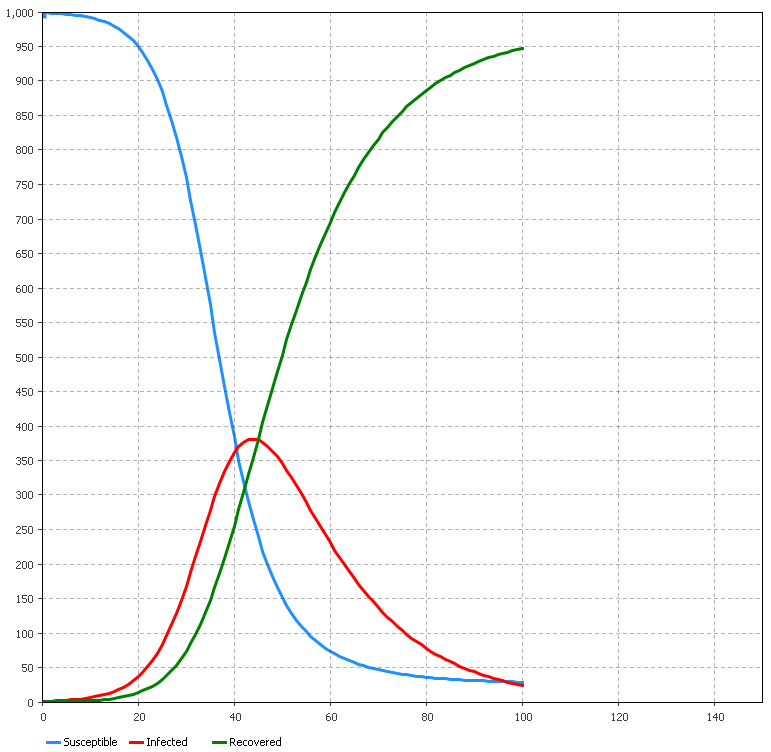
\includegraphics[width=.4\textwidth, angle=0]{./fig/SIR_SD_1000agents_100t_ANYLOGIC.png}
	\caption{System Dynamics simulation of SIR compartment model in AnyLogic Personal Learning Edition 8.3.1. Population Size $N$ = 1,000, contact rate $\beta = \frac{1}{5}$, infection probability $\gamma = 0.05$, illness duration $\delta = 15$ with initially 1 infected agent. Simulation run until $t = 100$.}
	\label{fig:sir_sd_anylogic}
\end{figure}